\chapter{Datos y Métricas}

    \noindent En este capítulo se van a presentar los datos de los que disponemos para resolver el problema principal de este trabajo (la identificación de landmarks cefalométricos mediante técnicas de few-shot learning), así como las principales métricas de error que se emplearán para estudiar la bondad de los resultados que se obtengan en futuros capítulos.

    \section{Datos del problema y framework empleado}
        \subsection{Base de datos proporcionada}
            \noindent El conjunto de datos Forense que se proporciona para resolver el problema presenta las siguientes características: 

            \begin{itemize}
                \item Contienen un total de \textbf{167 imágenes} de distintos sujetos. No se distribuye de forma equitativa el número de imágenes por sujeto, de manera que para algunos sujetos solo se dispone de una imagen mientras que otros disponen de varias. El sujeto con mayor número de imágenes tiene siete.
                \item La resolución de las imágenes también varía mucho, encontrando imágenes de alta calidad junto con otras con una muy baja resolución.
                \item Hay imágenes a color y en escla de grises.
                \item Las imágenes se presentan en un conjunto muy variado de posiciones. Disponemos de: 
                \begin{itemize}
                    \item $87$ imágenes frontales.
                    \item $57$ imágenes con rostros en posición de $3/4$.
                    \item $23$ imágenes de perfil.
                \end{itemize}
                \item Hay hasta un total de $30$ landmarks que pueden marcarse, aunque por regla general el número de landmarks en las imágenes es menor, como puede apreciarse en la \autoref{fig:Histograma}.
                \item En la \autoref{fig:Histograma} también podemos apreciar como la aparición de algunos landmarks es extremadamente baja, como es el caso del \textit{prosthion} y el \textit{Tragion} (tanto el izquierdo como el derecho). El resto de landmarks aparecen en más de la mitad de las imágenes. 
                \medskip
                \noindent La aparición en mayor o menor medida de cierto landmark en las imágenes nos sirve de indicador de si podrá ser o no aprendido por el modelo que usemos, de manera que los landmarks mencionados anteriormente, a causa del bajo número de ejemplos en los que aparecen puede ser más difícil que se aprendan.
            \end{itemize}


                \begin{figure}[!h]
                    \centering
                    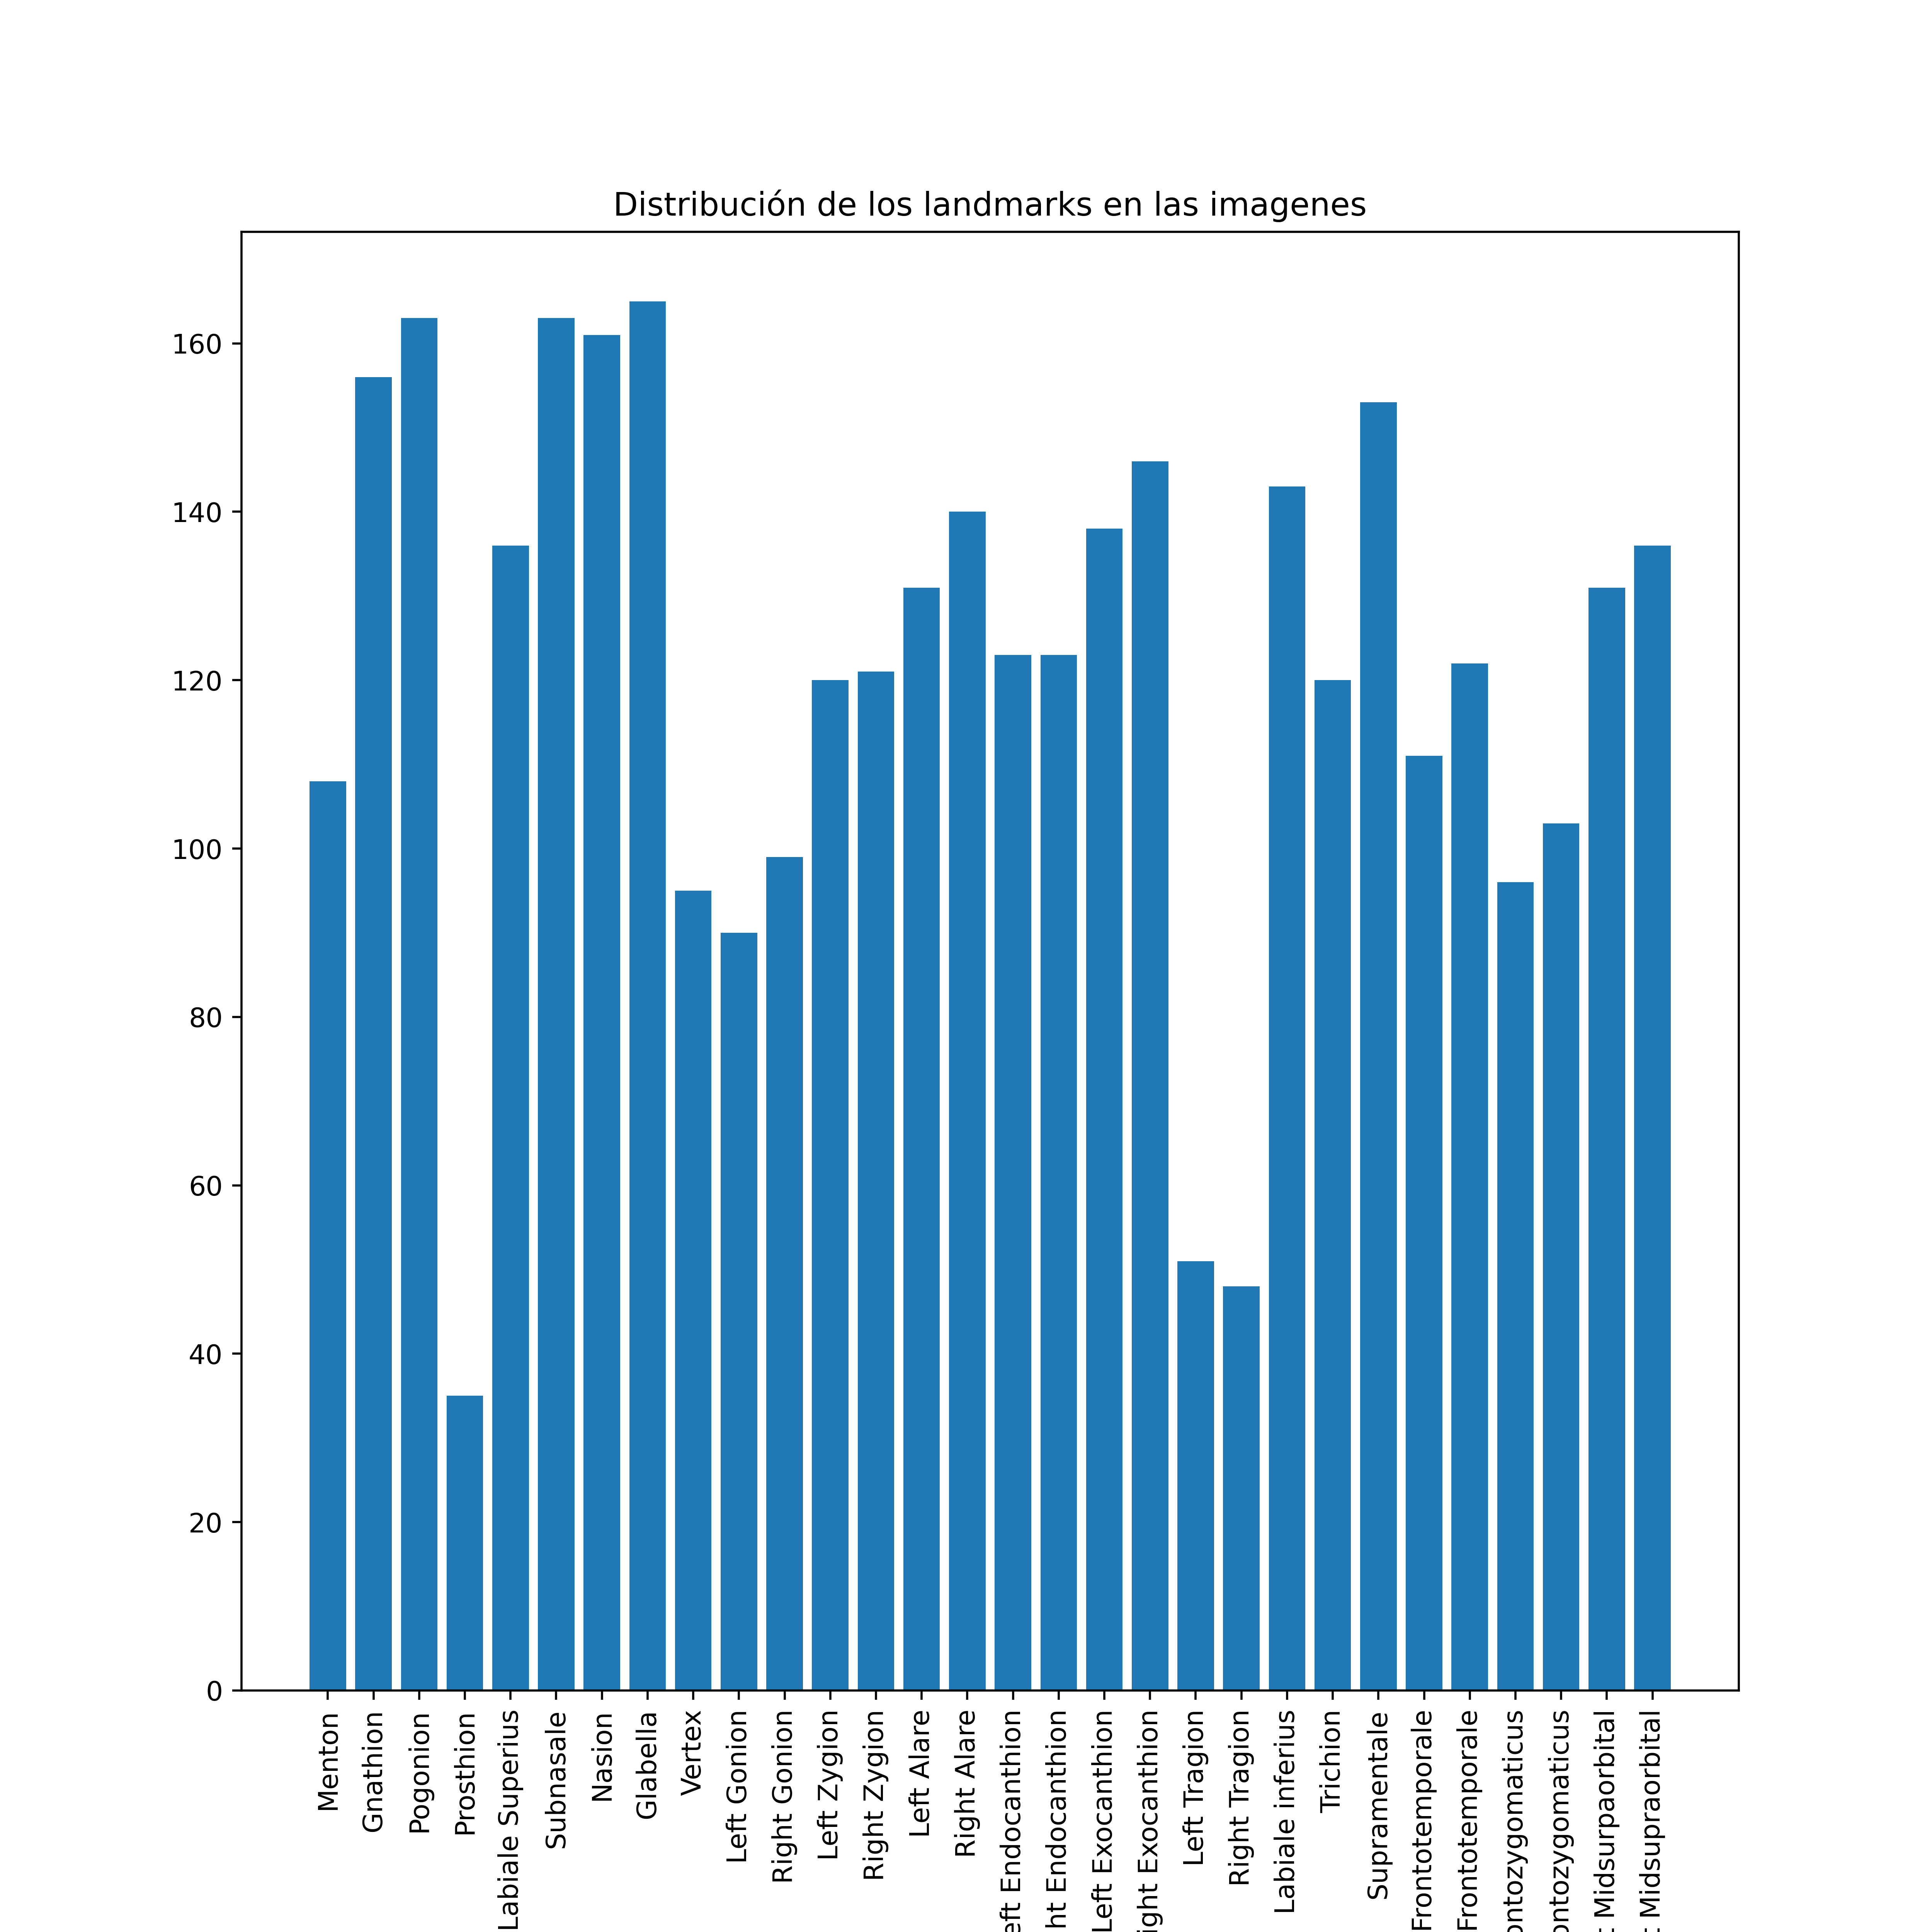
\includegraphics[width=0.7\textwidth]{img/distribucion_landmarks_imagenes.png}
                    \caption{Histograma con la aparición de cada tipo de landmark en las imágenes del dataset.}
                    \label{fig:Histograma}
                \end{figure}
                
        \subsection{Red empleada: 3FabRec}
            \noindent La red empleada para la resolución del problema es la desarrollada por \textbf{Bjorn Browatzki et al} en $2020$ \cite{browatzki20203fabrec} denominada \textbf{3FabRec}.La red en cuestión es un \textbf{Adversarial Autoencoder} que ha sido modificado para poder predecir landmarks incluyendo unas capas intermedias denominadas \textit{Interleaved Transfer Layer} en la etapa de reconstrucción y que explicaremos en profundidad más adelante.            

            \medskip

            \noindent Aplica un método \textit{semi-supervisado} en el cual:
            
            \begin{itemize}
                \item Hay una primera fase de \textbf{aprendizaje no supervisado} dónde se pretende adquirir conocimiento implícito sobre la estructura facial contenida en grandes conjuntos de imágenes de rostros de personas en diversas posiciones, iluminación y etnia. Para ello se codifica todo este conocimiento implícito en un vector de un espacio latente de baja dimensionalidad para posteriormente reconstruir la imagen. Este proceso se hace íntegramente en el \textit{Adversarial Autoencoder}.
                \item Posteriormente, en una segunda fase de \textbf{aprendizaje supervisado}, se entrena la red con un conjunto de imágenes etiquetadas con landmarks faciales que la red tratará de predecir. Para ello se intercalan entre las capas del generador capas de convolución encargadas de reconstruir los mapas de calor de cada landmark junto con la reconstrucción del rostro del paso previo.
                \item Finalmente, se puede incluir una tercera fase de \textit{finetuning} en la cual se entrena el Encoder para mejorar el rendimiento en la predicción de landmarks.
            \end{itemize} 

            \begin{figure}[!h]
                \centering
                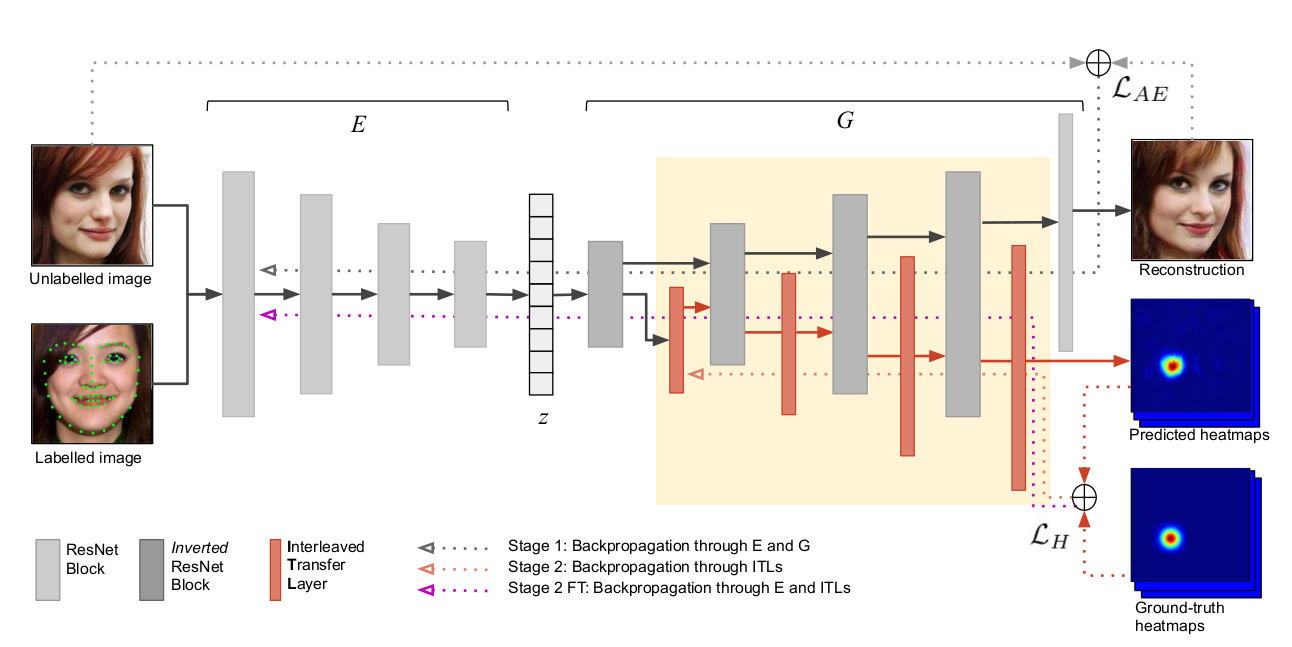
\includegraphics[width=0.7\textwidth]{img/3fabrec_arquitectura.png}
                \caption{Imagen resumen del framework 3FabRec. En ella podemos ver la estructura del \textit{Adversarial Autoencoder}, dividido en un Encoder (región bajo la \textit{E}) y un Generator (región bajo la \textit{G}) }
                \label{fig:3FabRec Resumen}
            \end{figure}

            \subsubsection{Arquitectura Adversarial Autoencoder}
                \noindent Para la construcción del \textit{Adversarial Autoencoder} emplean:
                
                \begin{itemize}
                    \item \textbf{Encoder}: emplean una ResNet-$18$  hasta codificar la entrada en un vector de $99$ dimensiones. Está pensado para imágenes de res $256 \times 256 \times 3$, aunque se adapta también a imágenes de dimensiones $512 \times 512 \times 3$.
                    \item \textbf{Decoder}: emplean la misma red ResNet-$18$ pero invertida.
                \end{itemize}

                \noindent Para una mejor comprensión he realizado unos diagramas con la herramienta \textit{diagrams.net}. En la \autoref{fig:bloque_encoder} podemos ver la estructura básica de los bloques de la ResNet-$18$.

                \begin{figure}[!h]
                    \centering
                    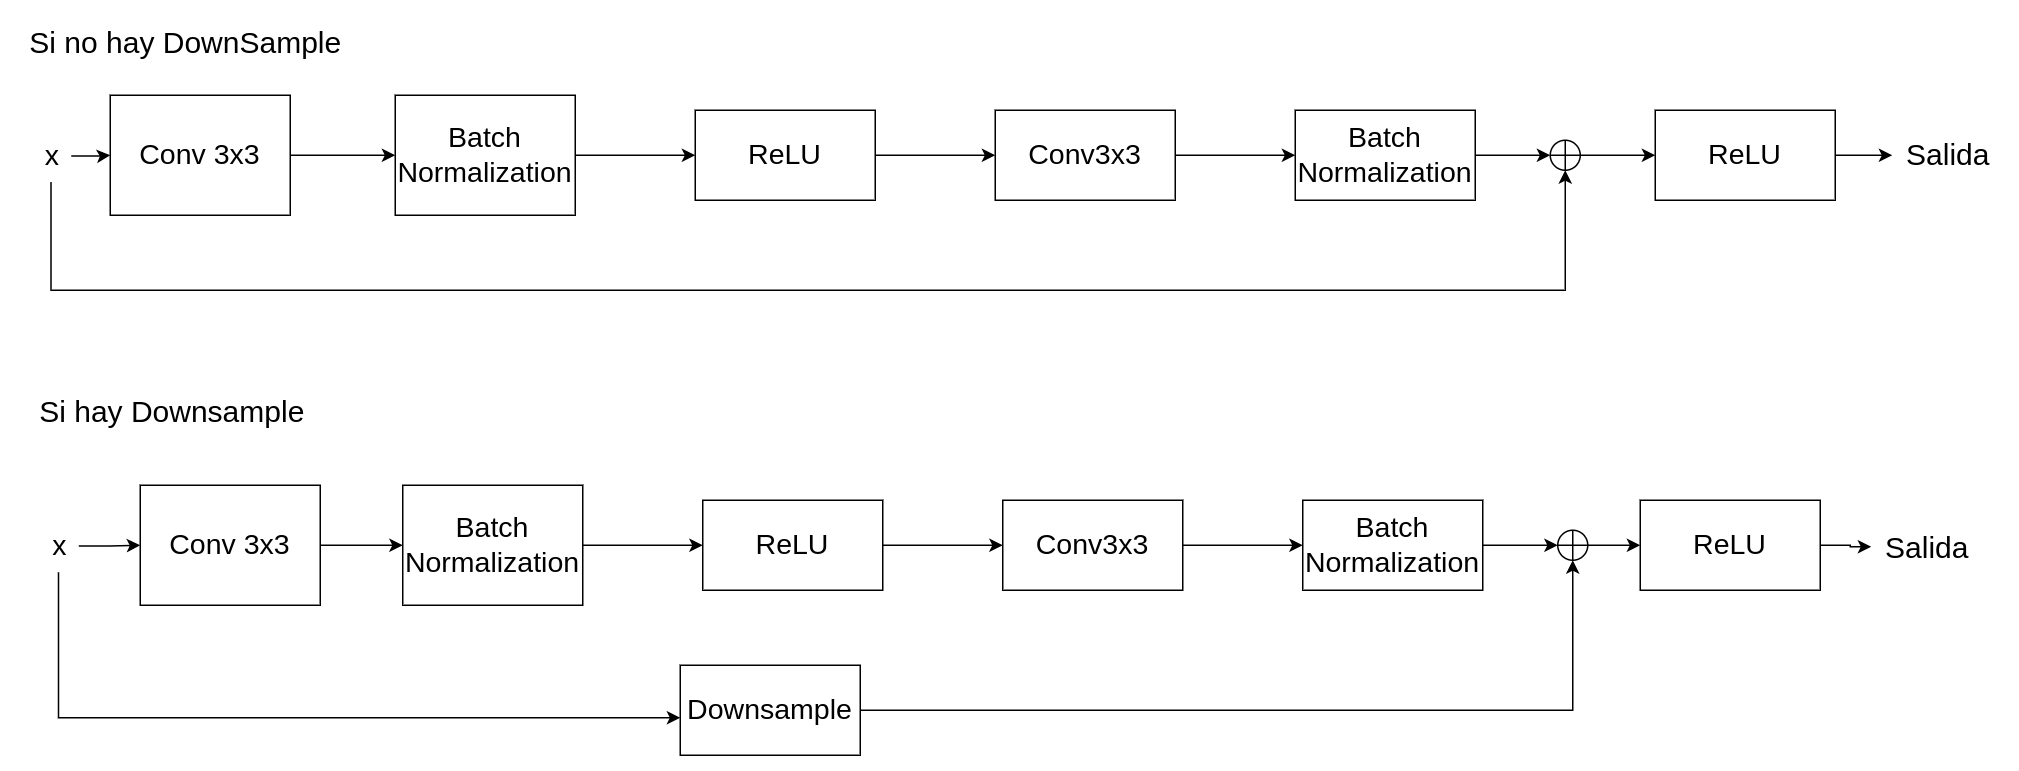
\includegraphics[width=0.7\textwidth]{img/bloque_basico_encoder.png}
                    \caption{Bloques básicos que utilza la red ResNet-$18$ en sus capas. Se trata de una sucesión clásica de Convolución 3x3 + Batch Normalization + ReLU que se repite dos veces. En el primer caso los filtros de convolución no reducen las dimensiones del tensor añadiendo un padding de 1. En el segundo caso se reduce la dimensión del tensor a la mitad tras la primera convolución y se manteiene la dimensionalidad en la segunda. En el primer caso, la suma residual puede realizarse con el tensor x sin problema, en el segundo caso el tensor debe reducirse para que casen las dimensiones.}
                    \label{fig:bloque_encoder}
                \end{figure}

                \medskip 

                \noindent Por otro lado en la \autoref{fig:Paso_encoder} podemos ver el paso de una imagen de entrada de tres canales y resolución $256 \times 256$ por el encoder.

                \begin{figure}[!h]
                    \centering
                    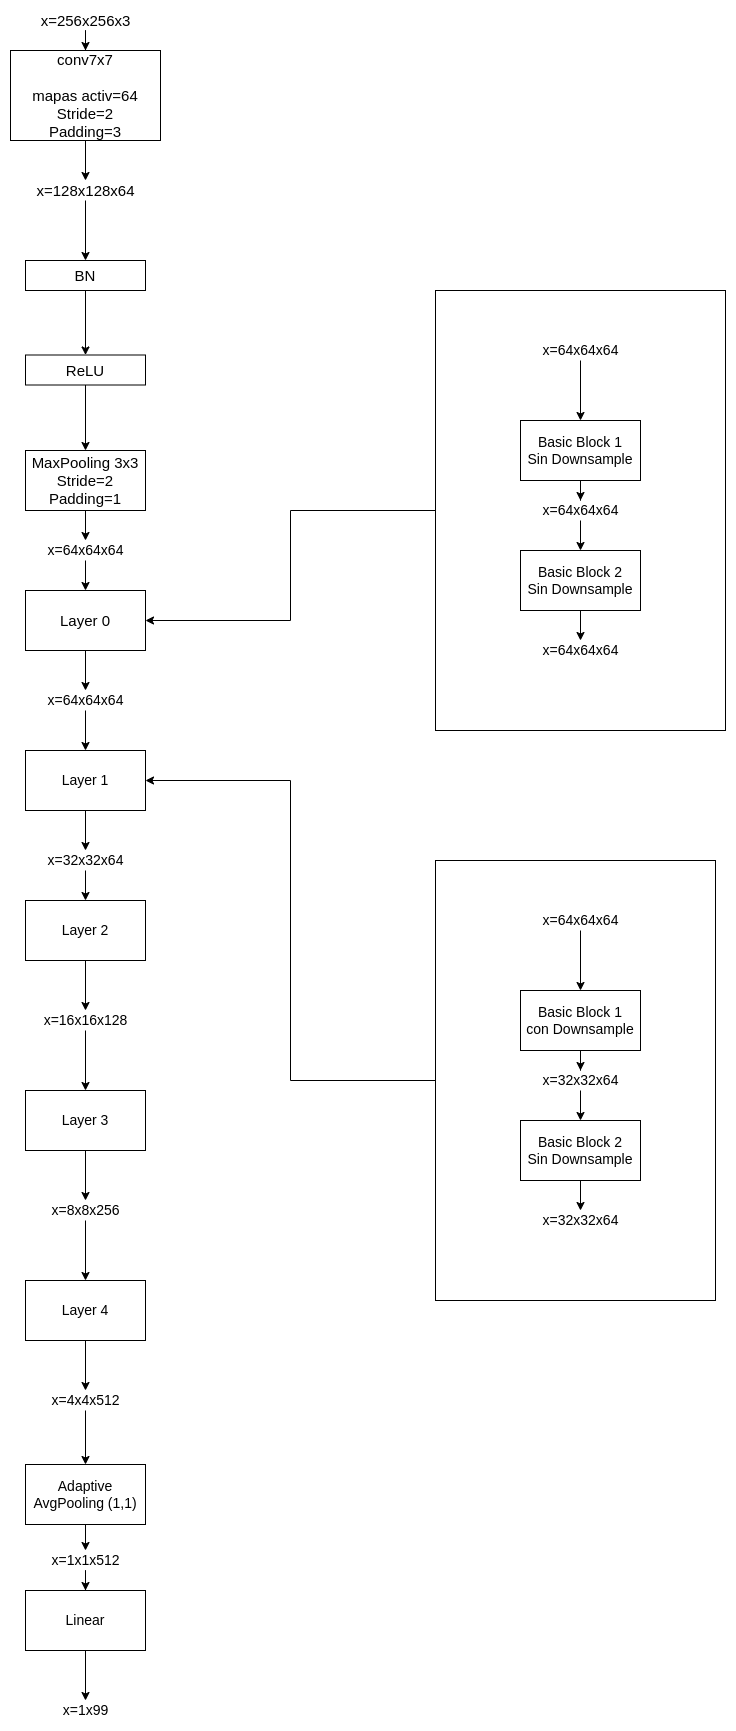
\includegraphics[width=0.7\textwidth]{img/3FabRec-Page-2.drawio.png}
                    \caption{Ejemplo de paso de una imagen a través del Encoder. Cabe destacar que a partir de la Layer 1, todos los bloques tienen downsample.}
                    \label{fig:Paso_encoder}
                \end{figure}

                \medskip

                \noindent En la \autoref{fig:Bloque_Decoder} podemos ver la estructura básica de un bloque en el Generador \textit{Inverse ResNet}, y un ejemplo del paso de un vector por el generador podemos verlo en la \autoref{fig:Paso_Generator}

                \begin{figure}[!h]
                    \centering
                    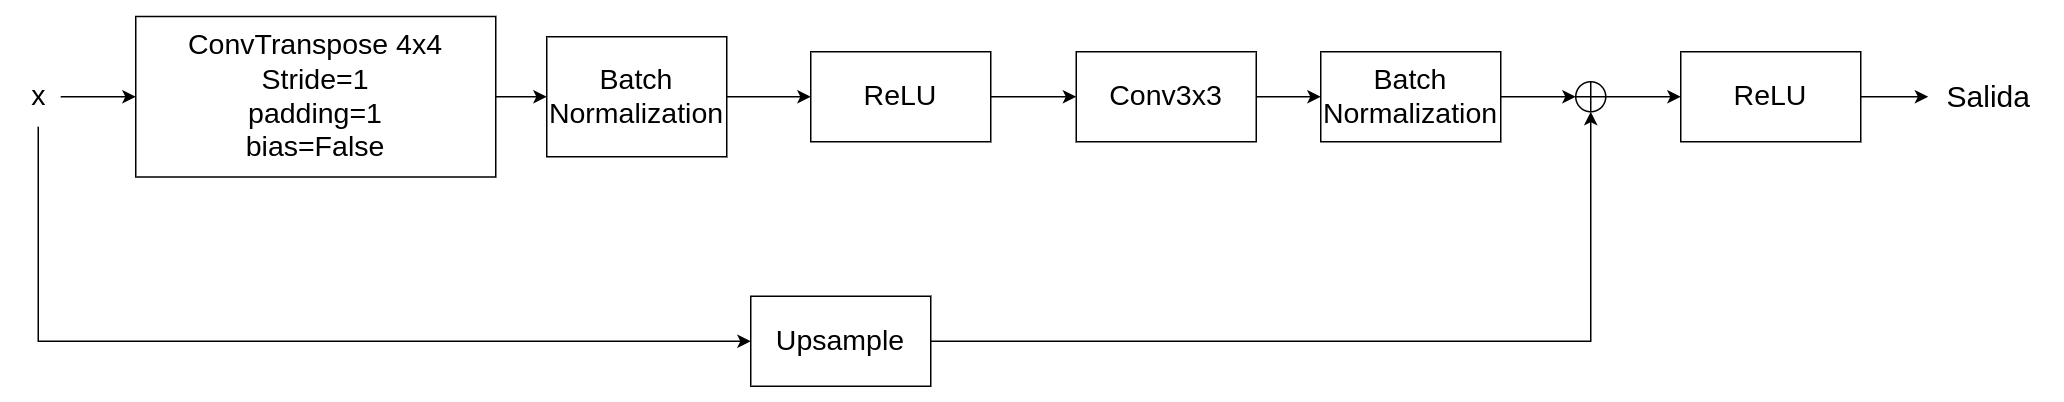
\includegraphics[width=0.7\textwidth]{img/bloque_invresnet.png}
                    \caption{En primer lugar se aplica una convolución transpuesta que duplica las dimensiones del tensor de entrada y tras esto se sigue la misma estructura que en el bloque básico de la ResNet-$50$, la segunda convolución $3\times 3$ mantiene las dimensiones. Como consecuencia, para sumar el tensor de entrada con la salida del bloque se aumentan las dimensiones de este.}
                    \label{fig:Bloque_Decoder}
                \end{figure}

                \begin{figure}[!h]
                    \centering
                    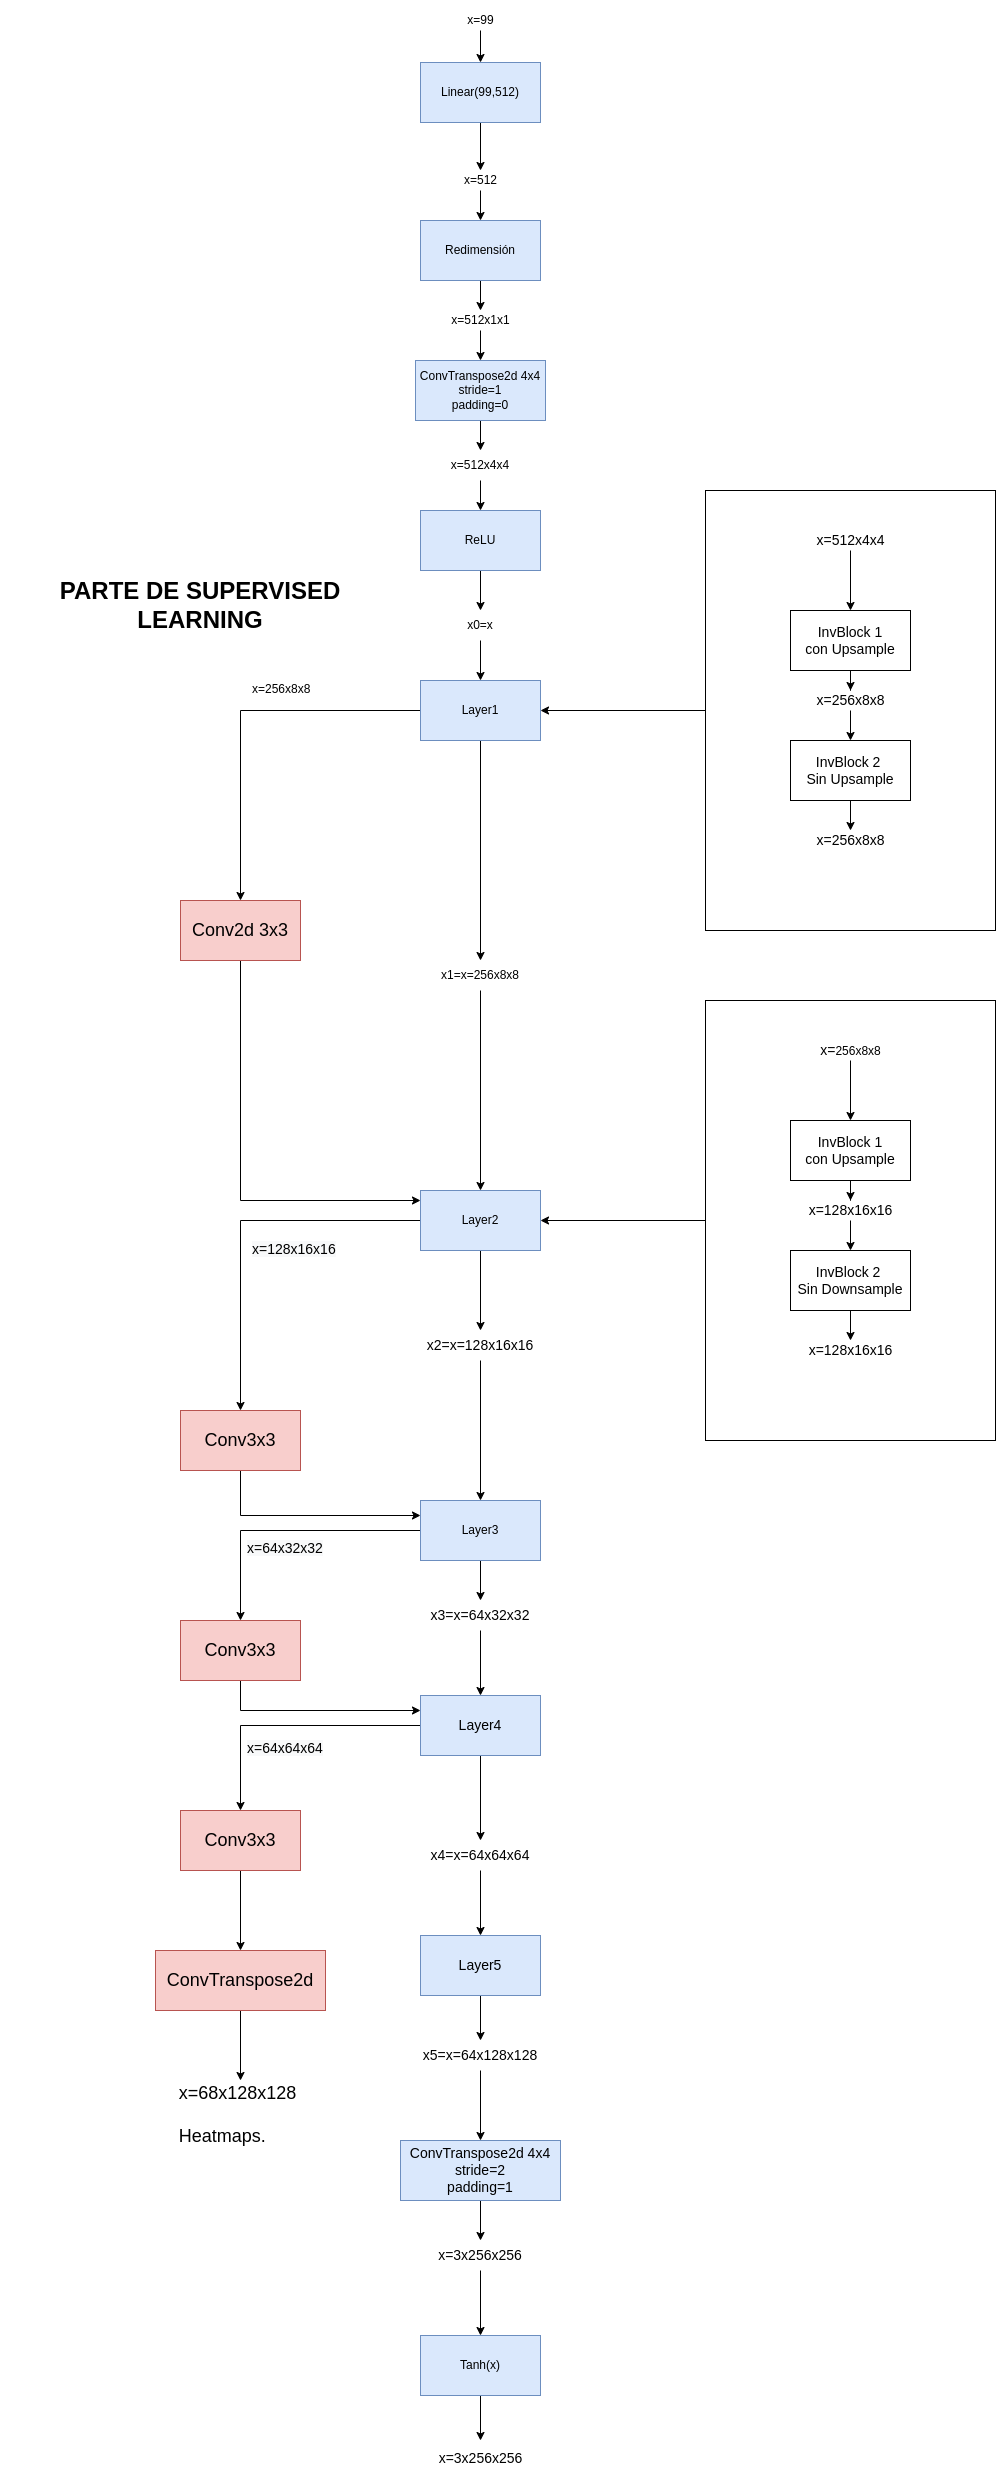
\includegraphics[width=0.5\textwidth]{img/paso_generator.png}
                    \caption{Ejemplo del paso de un vector de $99$ dimensiones por el generador hasta reconstruirse la imagen de dimensiones $256 \times 256 \times 3$. La parte correspondiente al aprendizaje supervisado es la de los cuadrados azules, los cuadrados rojos corresponden a las \textit{ITLS} de la parte supervisada que se intercalan entre cada dos capas y dan como resultado los mapas de calor de los landmarks predichos.}
                    \label{fig:Paso_Generator}
                \end{figure}

                \noindent Finalmente, para definir el autoencoder necesitamos un Discriminador, el cual que procure que los vectores del espacio vectorial latente sigan una determinada distribución. Dicha distribución será una normal multivariante estándar a la que vamos a añadirle un segundo discriminador propio de las redes \textbf{GAN} que nos dirá si la imagen reconstruida procede de la distribución que siguen los píxeles de la imagen de inicio. En la \autoref{fig:DGaussian} las redes neuronales que definen ambos discriminadores.

                \begin{figure}[!h]
                    \centering
                    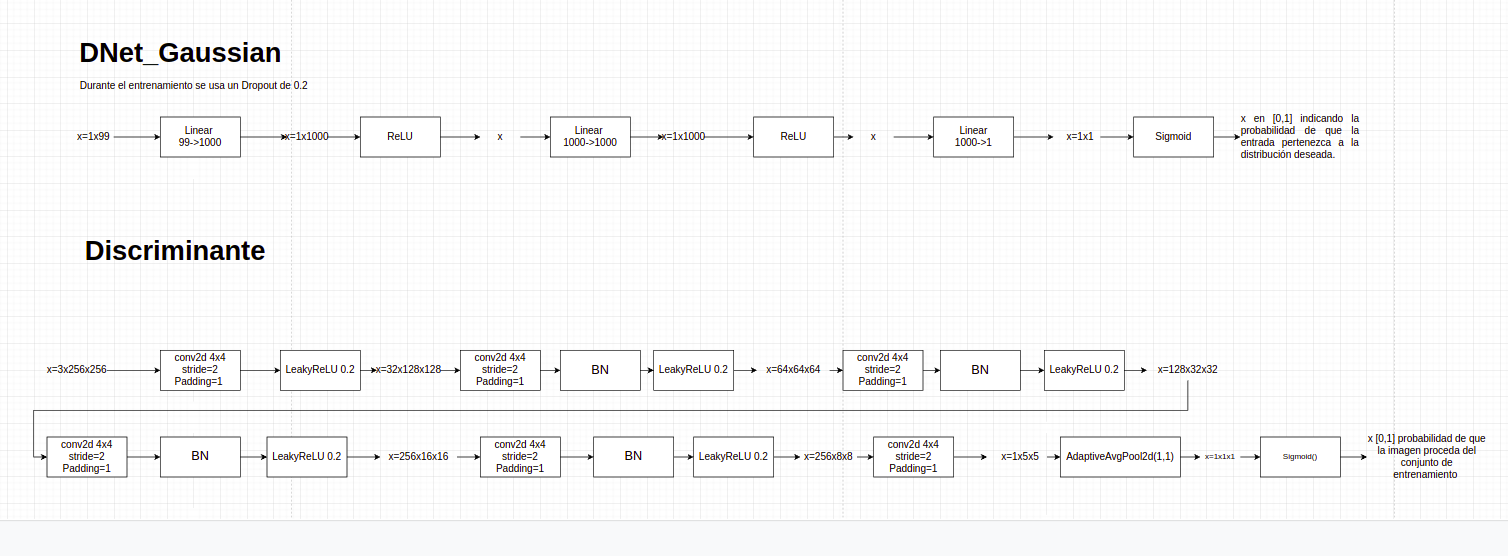
\includegraphics[width=0.99\textwidth]{img/DGaussian.png}
                    \caption{En la imagen superior vemos el discriminante que se emplea para los vectores producidos por el Encoder y en la imagen inferior vemos el discriminante que se emplea para las imágenes generadas por el Generador. En ambos casos se da como salida un valor entre $0$ y $1$ que hace referencia a la probabilidad de pertenecer a la distribución deseada en el primer caso o a seguir la distribución de los píxeles de las imágenes en el segundo caso.}
                    \label{fig:DGaussian}
                \end{figure}

            \subsubsection{Interleaved Transfer Layer (ITL)}
                
                \noindent Se tratan de simples capas convolucionales que se intercalan entre las capas del Generador. La última de estas capas proporciona como salida un conjunto de mapas de calor, uno por cada landmark predicho. Estos mapas de calor luego se emplean para representar en la imagen reconstruida los landmarks. La arquitectura de esta etapa podemos verla en la \autoref{fig:Paso_Generator}.
                
            \subsection{Función de pérdida}

                \noindent Para el entrenamiento de la red se emplean dos funciones de pérdida, la primera que presentaremos se emplea en el entrenamiento del \textit{Adversarial Autoencoder}, en la parte no supervisada, y la segunda función de pérdida se empleará tanto en la parte de aprendizaje supervisado como en la de \textit{finetuning} del Encoder.
        
                \medskip
        
                \noindent La función de pérdida empleada para el entrenamiento del \textit{Adversarial Autoencoder} en la parte de aprendizaje no supervisado es la siguiente: 
                
                \begin{align*}
                    \min_{E,G} \max_{D_z,D_x} & \mathcal{L}_{AE}(E,G,D_z,D_x) = \\
                    & \lambda_{rec} \mathcal{L}_{rec}(E,G) + \lambda_{cs}\mathcal{L}_{cs}(E,G) \\
                    & + \lambda_{enc}\mathcal{L}_{enc}(E,D_z)+ \lambda_{adv} \mathcal{L}_{adv}(E,G,D_x)
                \end{align*}

                \noindent En la cual $\lambda_{enc}$ y $\lambda_{adv}$ toman el valor $1.0$ mientras que $\lambda_{rec}$ y $\lambda{cs}$ se establecen en $1.0$ y $60.0$ respectivamente. El valor de la función de coste se propagará por los pesos de $E$,$G$,$D_z$ y $D_x$ actualizándolos mediante \textit{back-propagation}.

                \medskip

                \noindent Por otro lado, la función de pérdida que se empleará en el entrenmiento de las \textit{ITLs} será la siguiente: 

                \begin{equation} \label{eq::L2}
                    \mathcal{L}_H(ITL) = \mathbb{E}_{x ~ p(x)} \left[ \| H-ITL(a_1)\|_2 \right]
                \end{equation}

                \noindent Dónde $a_1$ serían los mapas de activación que genera el primer bloque de la ResNet invertida para la imagen codificada $z=E(x)$ (siendo $x$ la imagen de entrada a la red). En este caso se computa la distancia \textbf{$L_2$}entre los \textit{Heathmaps} de los lanmarks originales de la imagen $x$ de entrada, y los predichos por las \textit{ITLs}. Propagando el error por los pesos de las \textit{ITLS} solamente.

                \medskip

                \noindent A modo de aclaración, las imágenes etiquetadas con landmarks a la red suelen proporcionarse con el siguiente formato: 

                \begin{itemize}
                    \item Un archivo con la imagen sin etiquetar. 
                    \item Un archivo de texto plano con las coordenadas de cada landmark en la imagen.
                \end{itemize}

                \noindent Dados estos archivos, el framework, calcula para cada landmark proporcionado un mapa de calor en una imagen de tamaño $128 \times 128$ en el caso de que las imágenes de entrada sean de $256 \times 256$. Y es a ese conjunto de imágenes (una por cada landmark) a las que denominamos $H$ en la función anterior.

                \medskip

                \noindent Finalmente, en la etapa de \textit{fine-tuning} se computa la misma función de pérdida de antes, con la salvedad de que el error se propaga tanto por las \textit{ITLs} como por los pesos del \textit{Encoder}. Esto permite que el \textit{Encoder} se codifiquen con mayor precisión las imágenes y que se eliminen factores irrelevantes para la predicción de landmarks como son el género, el color de piel o la iluminación. Por otro lado se evita el overfitting ya que durante esta última etapa los pesos del \textit{Decoder} no se actualizan.
        
            \subsection{Proceso de entrenamiento de la red}

                \subsubsection*{Entrenamiento no-supervisado}
                    \noindent El framework que empleamos ha sido entrenado durante $50$ épocas con imágenes de tamaño $256x256$ y con un tamaño de batch de $50$. En todas las etapas del entrenamiento se ha empleado un optimizador tipo Adam, el cual durante el entrenamiento del \textit{Adversarial Autoencoder} usó $\beta_1=0.0$ y $\beta_2=0.999$ con un \textit{learning rate} de $2\times 10^{-5}$.

                    \medskip

                    \noindent Por otra parte, se aplicaron técnicas de \textit{data-augmentation} a las imágenes de entrada como giros horizontales, traslaciones, \textit{resizing} o rotaciones.

                \subsubsection*{Entrenamiento supervisado}
                    \noindent Para el entrenamiento de la parte supervisada, las imágenes de entrada se recortan de acuerdo a un \textit{bounding-box} creado por el framework a partir de unas coordenadas de entrada o bien de acuerdo a los landmarks que se proporcionan. Tras el recorte, se reescala la imagen hasta tener un tamaño de $256\times256$. 
                    
                    \medskip

                    \noindent Por otro lado se crean los \textit{Heathmaps} para cada landmark. Para esto se crea una imagen de tamaño $128 \times 128$ por cada landmark marcando el punto con ayuda de una distribución normalde dos dimensiones centrada en las coordenadas del landmark y usando un valor $\sigma=7$.

                    \medskip

                    \noindent Tras esto se entrenan las cuatro \textit{ITLs}. A los datos de entrada se les aplican técnicas de \textit{data-augmentation} como rotaciones, traslaciones, reescalados y oclusiones. Para esta etapa se usa también un optimizador Adam con un \textit{learning rate} de $0.001$ y los mismos valores para $\beta_1$ y $\beta_2$.

                    \medskip

                    \noindent Finalmente, durante la etapa de \textit{fine-tuning} se establece un \textit{learning-rate} de $0.0001$ en las \textit{ITLs} mientras que el del \textit{Encoder} se mantiene en su valor por defecto de $2 \times 10^{-5}$ y cambiando el valor de $\beta_1 = 0.9$.

            \subsection{Bases de datos usadas por el framework}
                
                \noindent Para el entrenamiento no supervisado se emplearon los siguientes datasets unidos: 

                \begin{itemize}
                    \item \textbf{VGGFace2} : Contiene un total de $3.3$ millones de imágenes de rostros en distintas poses, edad, iluminación, etnia, etc... Del dataset eliminaron las imágenes de rostros que tuviera una altura mayor a $100$ píxeles, quedando un total de $1.8$ millones de caras.
                    \item \textbf{AffectNet} : Se trata de un dataset de $228$ mil imágenes en una gran variedad de poses, iluminación, etc..
                \end{itemize}

                \noindent En total usaron unas $2.1$ millones de imágenes.

                \noindent Para el entrenamiento no supervisado se emplearon los siguientes datasets: 

                \begin{itemize}
                    \item \textbf{300-W} : une diversos datasets de rostros etiquetados con \textbf{$68$}landmarks de manera semi-automática como son \textbf{LFPW},\textbf{AFW}, \textbf{HELEN} y \textbf{XM2VTS}. Además de añadir datos propios. En total emplearon $3,148$ (aproximadamente el $80 \%$ )imágenes para el entrenamiento y $689$ para test, las cuales se dividieron en dos grupos, uno de $554$ imágenes considerado el grupo test estándar, y otro de $135$ imágenes difíciles.
                    \item \textbf{AFLW} : contiene un total de $24,386$ imágenes \textit{in-the-wild} con un amplio rango de poses distintas. Se emplearon $20,000$ (aproximadamente el $80 \%$) imágenes para test y $4,386$ para entrenamiento. Las imágenes vienen etiquetadas con $21$ landmarks, pero en el framework se entrena la red para predecir \textbf{$19$}.
                    \item \textbf{WFLW}: Es la más reciente de las empleadas y tiene un total de $10,000$ imágenes. Se usan $7,500$ para entrenamiento y $2,500$ para test. Las imágenes tienen un total de \textbf{$98$} landmarks anotados.
                \end{itemize}

    \section{Metricas}
        
        \noindent A conitnuación mostraremos las métricas empleadas para estudiar la bondad de los resultados. Algunas de estas métricas ya se emplearon en la funciones de coste del apartado anterior. 

        \subsection{SSIM}
            \noindent Se trata del \textit{structural similarity index} (SSIM) y da una medida de \textit{similaridad} entre dos imágenes \cite{wang2004image}, su expresión es la siguiente: 

            \begin{equation}
                SSIM(x,y)=[l(x,y)]^\alpha[c(x,y)]^{\beta}[s(x,y)]^{\gamma}
            \end{equation}

            \medskip

            \noindent Dónde $x,y$ son las dos imágenes que van a ser comparadas.

            \medskip

            \noindent La componente $c(x,y)$ hace referencia a la función de comparación del contraste de las dos imágenes y viene dada por la siguiente expresión: 

            \begin{equation}
                c(x,y)=\frac{2\sigma_x \sigma_y + C}{\sigma_x^2+ \sigma_y^2+C}
            \end{equation}

            \noindent Dónde $\sigma_x, \sigma_y$ hacen referencia a la desviación estándar de cada imagen.

            \medskip

            \noindent La componente $s(x,y)$ es la función de comparación estructural entre las dos imágenes y viene dada por la siguiente expresión:

            \begin{equation}
                s(x,y)=\frac{\sigma_{xy}+C/2}{\sigma_x \sigma_y +C/2}
            \end{equation}

            \noindent Dónde $\sigma_{xy}$ denota la covarianza.

            \medskip

            \noindent La componente $l(x,y)$ hace referencia a la \textit{luminosidad}, pero en el caso de 3FabRec se prescinde de esta componente, además los exponentes $\alpha, \beta , \gamma$ se igualan a $1$.

            \medskip

            \noindent Por otra parte siguen las indicaciones del paper original de SSIM que recomiendan usar estas comparaciones en regiones de la imagen y promediarlas en vez de aplicarlas sobre todo el conjunto de píxeles de la imagen, es por ello que la expresión final queda:

            \begin{equation}
                cs(x,y)=\frac{1}{|w|} \sum{c(x_w,y_w)s(x_w,y_w)}_w
            \end{equation}

            \noindent Dónde $w$ representa la ventana sobre la que se aplica la función y $|w|$ el total de ventanas. En nuestro caso se emplean ventanas de tamaño $31\times 31$.

        \subsection{Average pixel error}
            \noindent Se trata de la función de coste \textbf{L1} que se aplica a la imagen original y la reconstruida  y nos porporciona una medida del error de reconstrucción a nivel de pixel. Este error se obtiene para cada imagen y luego se devuelve el error promedio, por eso se denomina \textit{Average pixel error}.

        \subsection{MSE}
            \noindent Se trata de la función de coste \textbf{L2} usada para medir la diferencia entre los mapas de calor pertenecientes a los landmarks reales y los mapas de calor de los landmarks predichos.Su expresión es \eqref{eq::L2}


\endinput
%------------------------------------------------------------------------------------
% FIN DEL CAPÍTULO. 
%------------------------------------------------------------------------------------

